The algorithm runs with different time on the three test problems. 


Initial values used on the test problems:      
\begin{align*}
		A &= 0.1*ones(m,1) \\
        q &= 0.1*ones(m,1) \\
        f_{supp} &= 10000*ones(3*ns,1) \\
        \lambda &= 10*ones(3*n,1) \\
\end{align*}   

On the tower problem, the algorithm was fast, with a running time of 0.20 seconds and 31 iterations. On the cantilever, it performed a litter lower, but still with running time of 0.58 seconds and 86 iterations. The bridge problem was outside the feasible set at these settings, so $A = 1.01*ones(m,1)$ was used instead. Here, the algorithm had a running time of 1.12 seconds and 114 iterations for the bridge problem. The tower used 47 iterations and the cantilever used 114 iterations for this initial value. 

The MATLAB functions spdiag, sparse, spalloc, speye and the back-slash operator were used to save memory and shorten run-time. The algorithm performed well for all the test problems, and seldom shortened the step length $\alpha$ more than two times, as predicted by the theory. 

The line search algorithm is presented here:

\begin{lstlisting}
function [A, q, f_supp] = SQP_lineSearch(A,q,f_supp)
  
    global m ns pen par rho l lambda p M A_top A_bottom
    eta = 0.25;
    iter = 0;
    p = zeros(2*m+3*ns,1);

    % Run while KKT-conditions not yet satisfied:
    while convergence(A, q, f_supp, lambda, p) > 0.001 && iter < 5000 
        
        iter = iter + 1;
        
        % Compute p and lambda_hat by solving (18.9)
        sol = solve_newton(A, q, f_supp);
        
        p = sol(1:2*m+3*ns);
        lambda_hat = sol(2*m+3*ns+1:end);
        p_lambda = lambda_hat - lambda;
        
        % Choose penalty parameter to satisfy (18.36) with sigma evaluated:
        pen = 0.5;
        % Parameter in (0,1):
        par = 0.5;

        % Sigma, is 1 if Hessian of L is pos. def.
        [~,posDef] = chol(hess_L(A,q));
        if posDef == 0
            sigma = 1;
        else
            sigma = 0;
        end

        % Penalty parameter must satisfy (18.36) by some margin:
        while pen*1.1 < (grad_f(A,q)'*p + sigma/2*p'*hess_L(A,q)*p)/((1-par)*norm(c(q, f_supp),1))
            pen = pen*1.1;
        end

        alpha = 1;
        i = 1;
            
%       alpha_store(1) = alpha;
        alpha_new = alpha;
        
        % Control that alpha*p leads to a more optimal point in the
        % feasible set:
        while ~isValid(alpha_new,eta, A, q, f_supp) || (M-sum(rho*l(:,3).*(A+alpha_new*p(1:m)))) < 0 || 
         ~isempty(find(((A+alpha_new*p(1:m))-A_bottom).*
         (A_top-(A+alpha_new*p(1:m))) < 0))

            % Reduce step length by a half
            alpha_new = alpha_new*0.5;
            
            % If it is not possible to choose alpha to satisfy all
            % criteria:
            if i > 1000
                error('initial conditions outside feasible set')
            end
            i = i + 1;
        end
        alpha = alpha_new;

        % Update A, q, f_supp and lambda with new step length:
        A = A + alpha*p(1:m);
        q = q + alpha*p(m+1:2*m);
        f_supp = f_supp + alpha*p(2*m+1:2*m+3*ns);

        lambda = lambda + alpha*p_lambda;   
            
    end
end
\end{lstlisting}

  
\begin{figure}[H]
\centerline{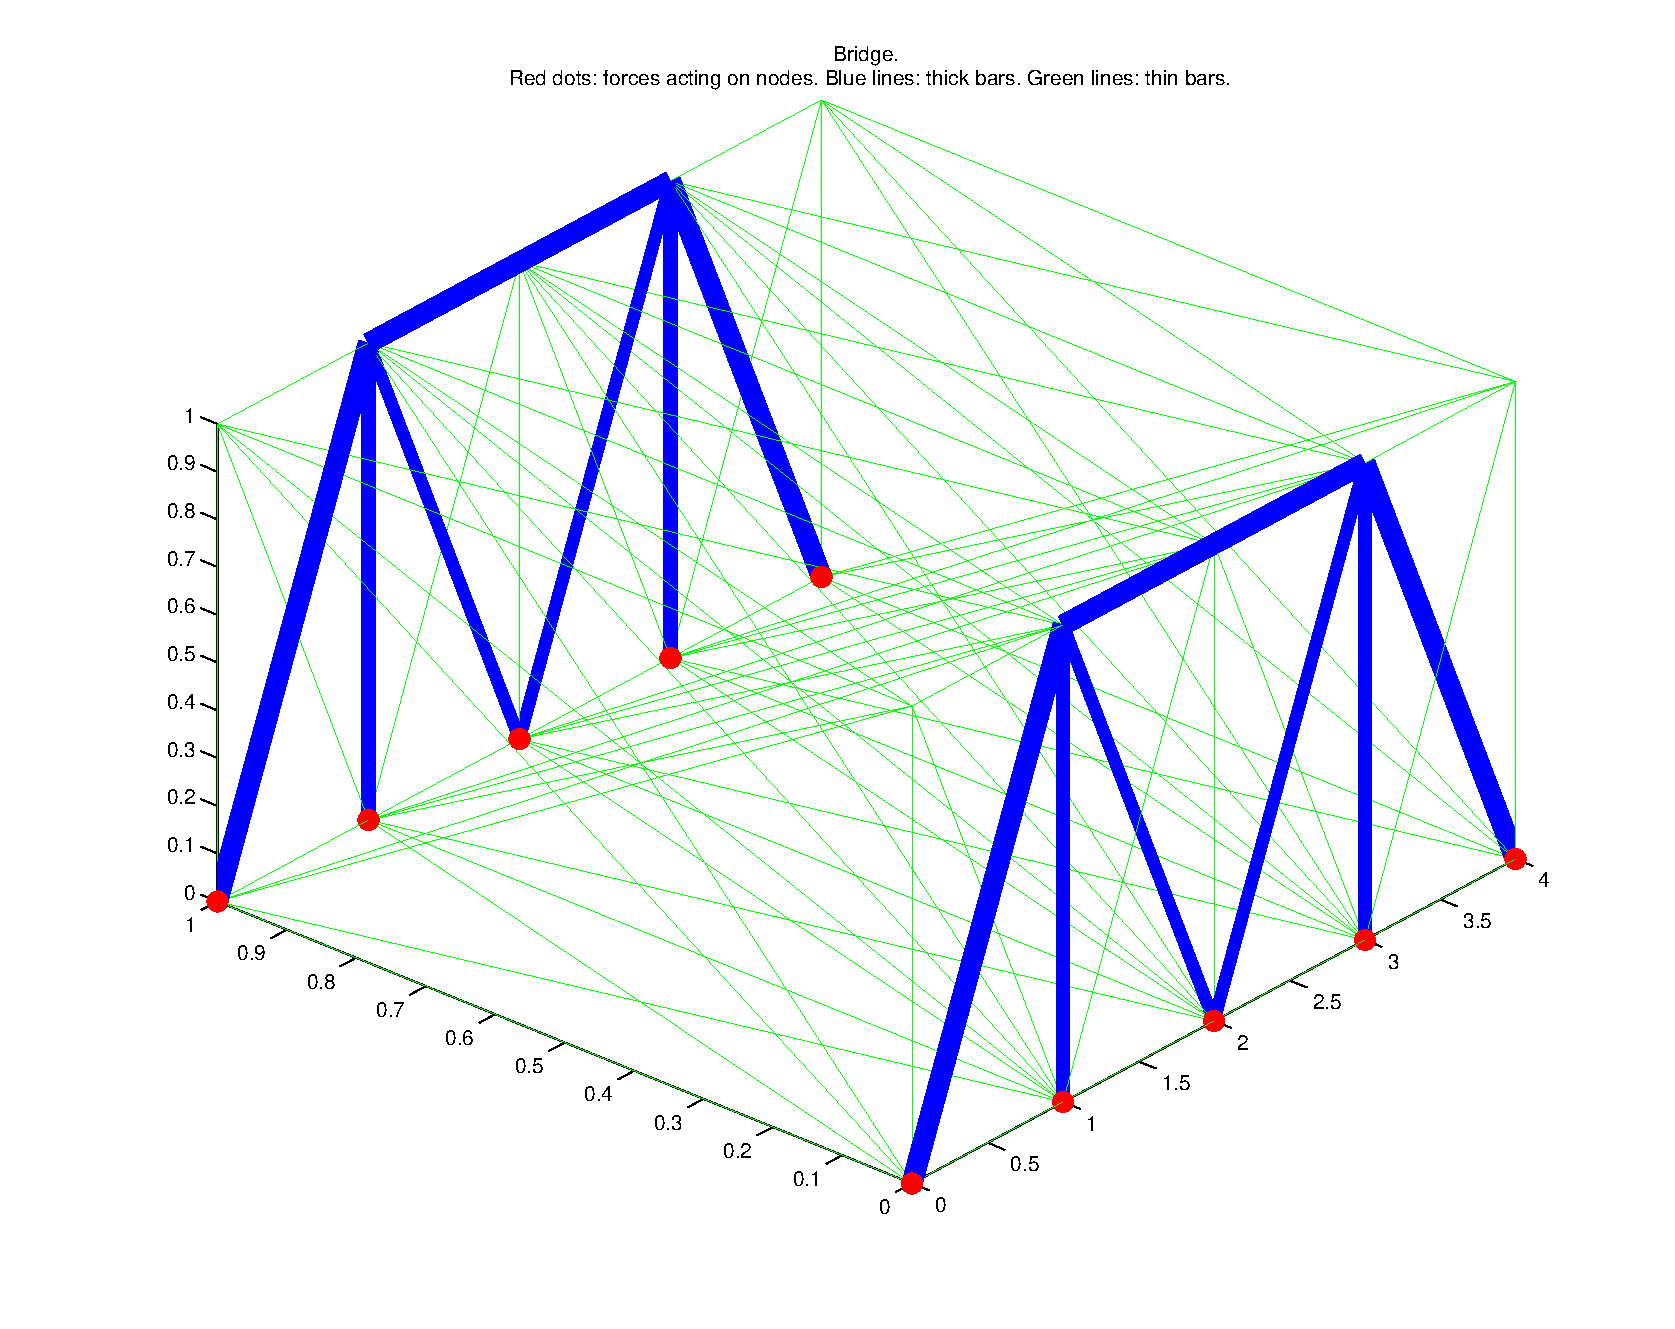
\includegraphics[scale=0.4]{../Ferdig kode/bridge.pdf}}
\caption{The bridge structure}
\label{fig:bridge}
\end{figure}

\begin{figure}[H]
\centerline{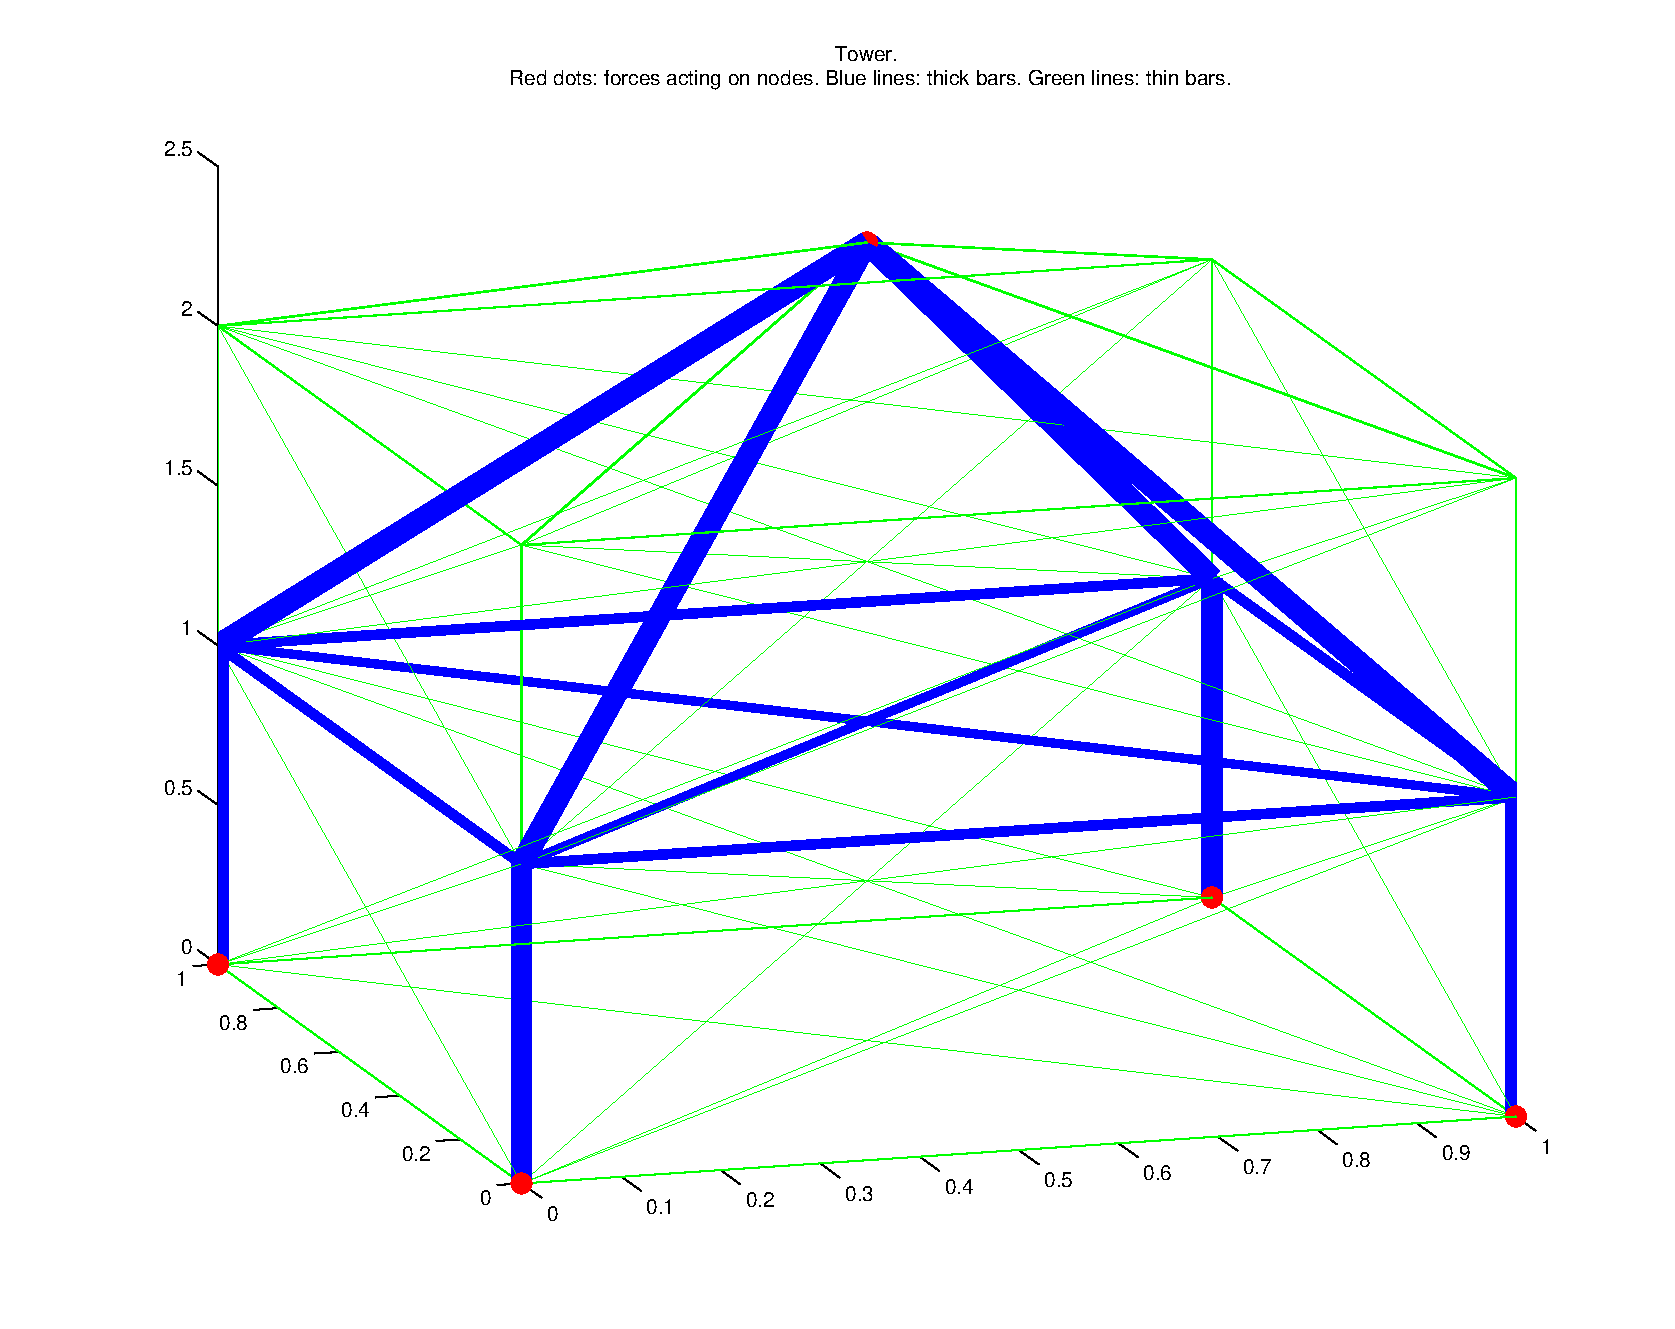
\includegraphics[scale=0.4]{../Ferdig kode/tower.pdf}}
\caption{The tower structure}
\label{fig:tower}
\end{figure}

\begin{figure}[H]
\centerline{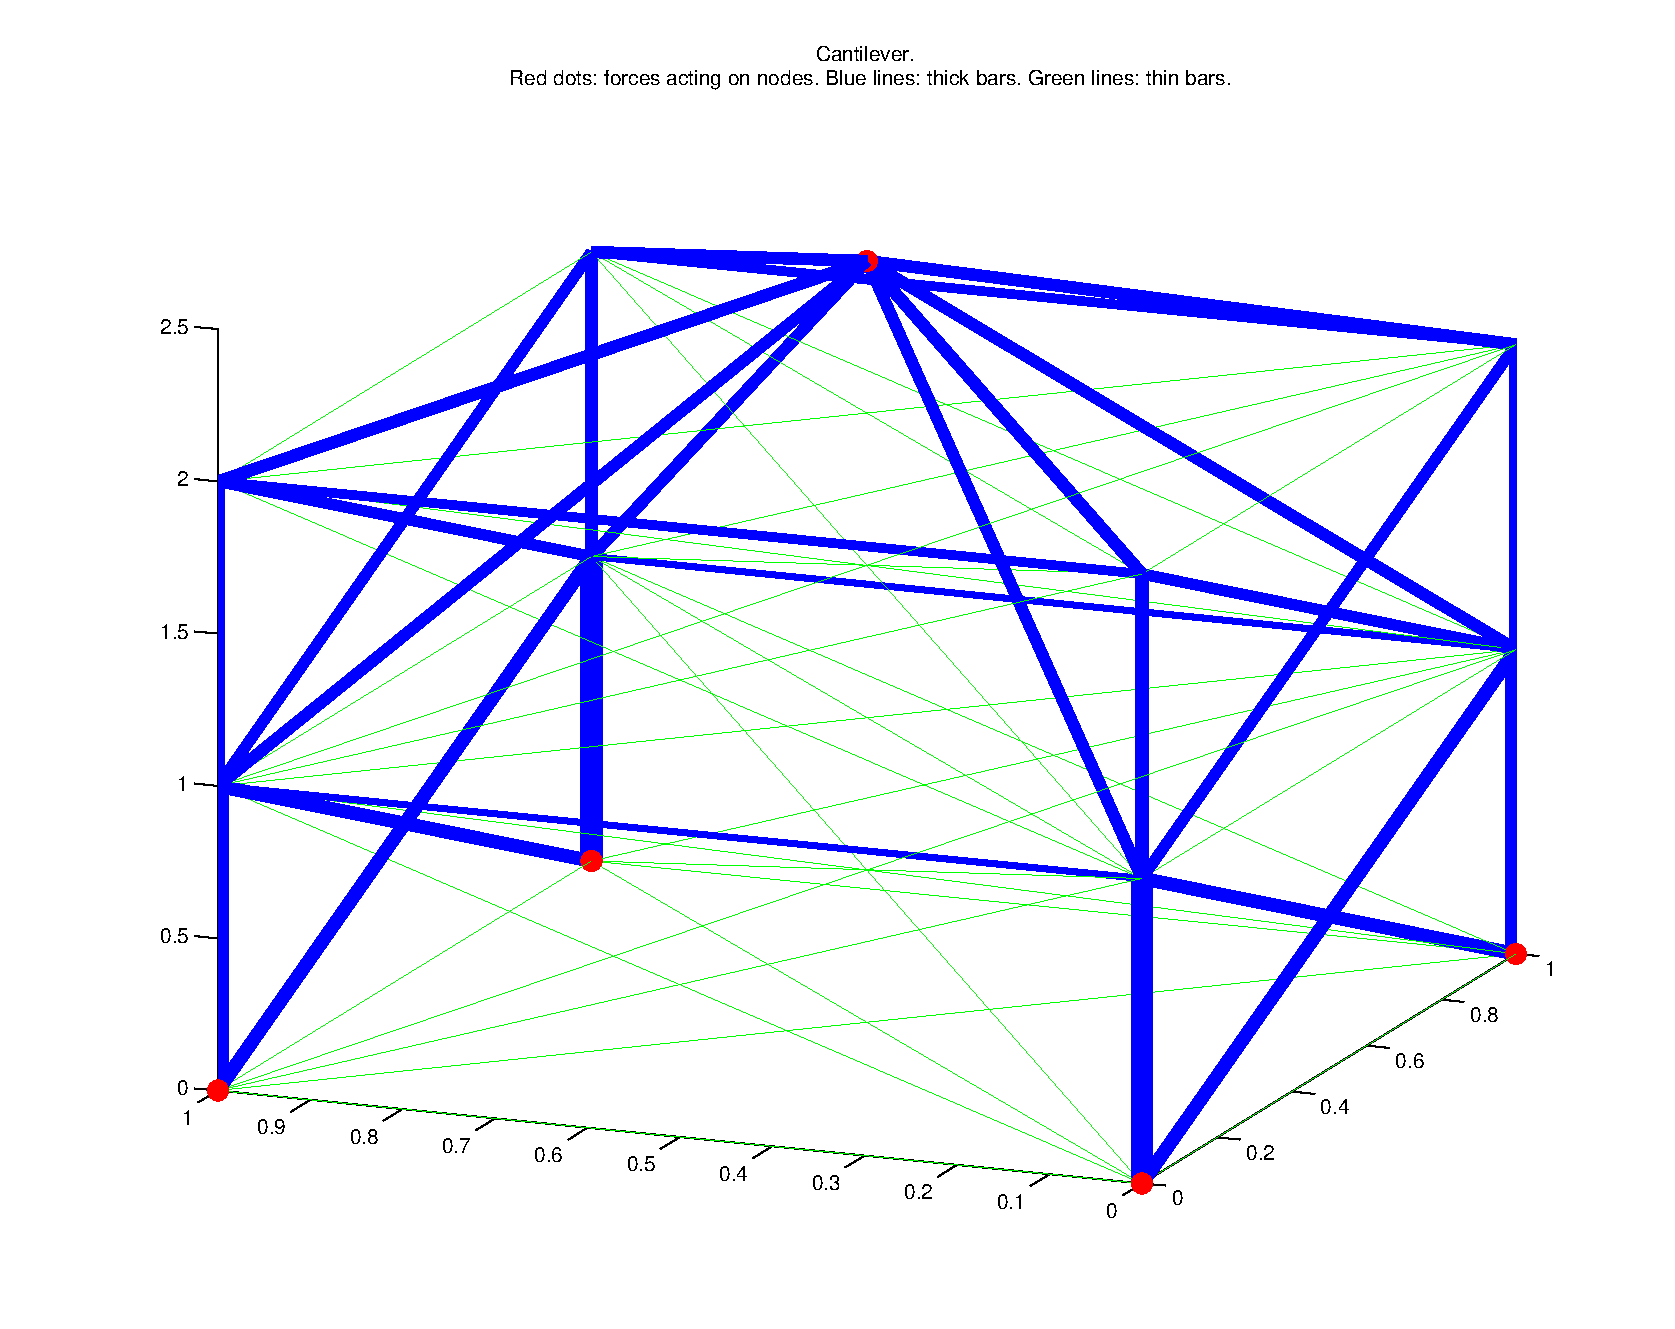
\includegraphics[scale=0.4]{../Ferdig kode/cantilever.pdf}}
\caption{The cantilever structure}
\label{fig:cantilever}
\end{figure}